%\documentclass[handout]{beamer}
%\usepackage{pgfpages}
%\pgfpagesuselayout{4 on 1}[a4paper, landscape, border shrink=5mm]
%\pgfpageslogicalpageoptions{1}{border code=\pgfusepath{stroke}}
%\pgfpageslogicalpageoptions{2}{border code=\pgfusepath{stroke}}
%\pgfpageslogicalpageoptions{3}{border code=\pgfusepath{stroke}}
%\pgfpageslogicalpageoptions{4}{border code=\pgfusepath{stroke}}
\documentclass{beamer}
%\usetheme{nesl}  % Now it's a beamer presentation with the NESL theme!
\usetheme{Warsaw}
\usepackage{tikz}
\usetikzlibrary{shapes,arrows}
\usepackage{url}
\usepackage{movie15}
\usepackage{verbatim}
\usefonttheme{serif}

% Make a new command that will make a new subsection and a frame with the same title
\newcommand{\fst}[2]{\subsection{#1}\frame{\frametitle{#1} #2}}

% Standard LaTeX stuff - note the optional abbreviated title being provided
\title{ACAPS final report 3.b and 3.c}
\subtitle{  3.b) Continue the developments and optimization of the WRF TL/ADJ code \\3.c)Maintain and perform regression testing of 4D-Var data assimilation code}

\date{~\\ \today ~\\
 ~\\
  ~\\
  ~\\
  ~\\
 \tiny{NCAR is sponsored by the National Science Foundation}
}

\institute[NCAR Earth System Laboratory]{
% \url{xinzhang@ucar.edu} \\
   NCAR Earth System Laboratory \\
%  \url{ook@ucw.cz}\\
%  Charles University, Prague
}

% We want the NSF department logo
\logo{
\includegraphics[height=.5in]{NESL.jpg}}


\begin{document}

% The title page
\frame{\titlepage}

%%%%%%%%%%%%%%%%%%%%%%%%%%%%%%%%%
\section{3.b) Continue the developments and optimization of the WRF TL/ADJ code. }

\fst{Upgrading WRFPLUS}{
\begin{itemize}
   	\item New WRF adjoint and tangent linear codes based on the latest WRF repository codes. \pause
	\item Constructed interfaces through which other applications can call WRF adjoint and tangent linear model directly. \pause 
	\item Testing the code on various  platforms and compilers ( IBM, Linux, Mac : xlf, g95, pgi, intel, gfortran). \pause
	\item Capability to do tangent linear and adjoint test over any length of time window. \pause 
	\item New WRFPLUS can be used as a standalone tool or as a component in 4D-Var system.
\end{itemize}
}

\begin{frame}[fragile]
\frametitle{Sample Tangent Linear and Adjoint Check of WRFPLUS }
\setbeamercolor{postit}{fg=black, bg=yellow}
\begin{beamerboxesrounded}[ lower=postit,shadow=true]{Tangent linear check:6 hours}
{\tiny
\begin{verbatim}
alpha_m=.1000E+00  coef=   0.98186174930325E+00  val_n= 0.3725210E+11  val_l= 0.3794027E+11
alpha_m=.1000E-01  coef=   0.99807498026522E+00  val_n= 0.3786723E+09  val_l= 0.3794027E+09
alpha_m=.1000E-02  coef=   0.99970559707666E+00  val_n= 0.3792910E+07  val_l= 0.3794027E+07
alpha_m=.1000E-03  coef=   0.99992019503144E+00  val_n= 0.3793724E+05  val_l= 0.3794027E+05
alpha_m=.1000E-04  coef=   0.10000447262220E+01  val_n= 0.3794196E+03  val_l= 0.3794027E+03
alpha_m=.1000E-05  coef=   0.99999981575068E+00  val_n= 0.3794026E+01  val_l= 0.3794027E+01
alpha_m=.1000E-06  coef=   0.99999998152933E+00  val_n= 0.3794027E-01  val_l= 0.3794027E-01
alpha_m=.1000E-07  coef=   0.99999990980017E+00  val_n= 0.3794026E-03  val_l= 0.3794027E-03
alpha_m=.1000E-08  coef=   0.99999956711797E+00  val_n= 0.3794025E-05  val_l= 0.3794027E-05
alpha_m=.1000E-09  coef=   0.10000030220656E+01  val_n= 0.3794038E-07  val_l= 0.3794027E-07
alpha_m=.1000E-10  coef=   0.99996176999678E+00  val_n= 0.3793882E-09  val_l= 0.3794027E-09
\end{verbatim}
}
\end{beamerboxesrounded}
\begin{beamerboxesrounded}[ lower=postit,shadow=true]{Adjoint check: 6 hours}
{\tiny
\begin{verbatim}
 ad_check: VAL_TL:    0.42476489986911E+11
 ad_check: VAL_AD:    0.42476489986912E+11
\end{verbatim}
}
\end{beamerboxesrounded}
\end{frame}

\section{3.c)Maintain and perform regression testing of 4D-Var data assimilation code}

\subsection{Single executable 4D-Var}
\begin{frame}[fragile]
\frametitle{Single executable 4D-Var}
WRFPLUS includes WRF NL, AD and TL model and they are used as a subroutine in WRF 4D-Var, other than being called via shell scripts.
~\\
~\\
\setbeamercolor{postit}{fg=black, bg=yellow}
\begin{beamerboxesrounded}[ lower=postit,shadow=true]{Nonlinear call}
\begin{verbatim}
old         call da_system ("da_run_wrf_nl.ksh")
new         call da_nl_model
\end{verbatim}
\end{beamerboxesrounded}
\begin{beamerboxesrounded}[ lower=postit,shadow=true]{Tangent linear call}
\begin{verbatim}
old         call da_system ("da_run_wrfplus_tl.ksh")
new         call da_tl_model
\end{verbatim}
\end{beamerboxesrounded}
\begin{beamerboxesrounded}[ lower=postit,shadow=true]{Adjoint call}
\begin{verbatim}
old         call da_system ("da_run_wrfplus_ad.ksh")
new         call da_ad_model
\end{verbatim}
\end{beamerboxesrounded}
\end{frame}

\begin{frame}[fragile]
\frametitle{Memory exchange}
The information (TL perturbation, adjoint forcing, basic states and gradient) is exchanged via linked lists.
~\\
~\\
\setbeamercolor{postit}{fg=black, bg=yellow}
\begin{beamerboxesrounded}[ lower=postit,shadow=true]{Read basic states}
\begin{verbatim}
call domain_clock_get( grid, current_timestr=timestr )
call da_read_basicstates ( xbx, grid, ... )
\end{verbatim}
\end{beamerboxesrounded}
\begin{beamerboxesrounded}[ lower=postit,shadow=true]{Save TL perturbation}
\begin{verbatim}
call push_tl_pert (timestr)
\end{verbatim}
\end{beamerboxesrounded}
\begin{beamerboxesrounded}[ lower=postit,shadow=true]{Save AD forcing}
\begin{verbatim}
call push_ad_forcing (timestr)
\end{verbatim}
\end{beamerboxesrounded}
\end{frame}

\frame{
\frametitle{Parallel run using all processors}
4D-Var is a sequential algorithm. However, the current parallel WRF 4D-Var constructed on the Multiple Program Multiple Data mode, which have to split the total processors into 3 subsets for DA, NL and AD/TL. Lots of CPU time are wasted
\begin{center}
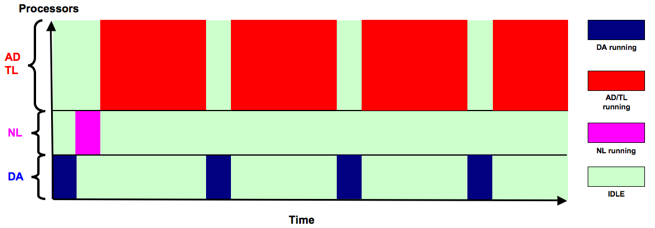
\includegraphics[scale=0.5]{mpmd_wrf4dvar}
\end{center}
}

\frame{
\frametitle{Parallel run using all processors}
Benefit from the single executable framework, every CPU is working at any time. No IDLE any more.
\begin{center}
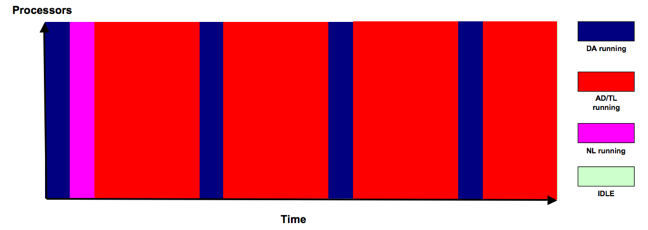
\includegraphics[scale=0.5]{single_exe_wrf4dvar}
\end{center}
}

\frame{
\frametitle{Performance improvement WRF 4DVar framework only}
\begin{itemize}
	\item $90x60x41@60km$, 6h window, 1h obs\_bin
	\item 27 iterations FGAT, NCAR bluefire (IBM P6)
\end{itemize}
\begin{center}
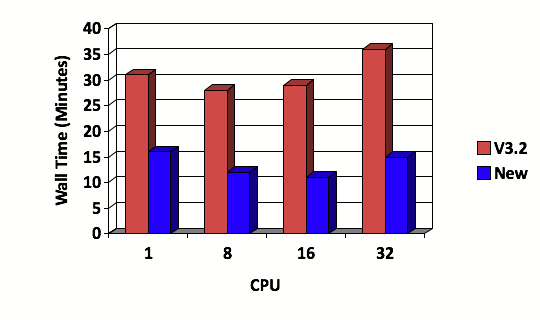
\includegraphics[scale=0.5]{small_case_performance}
\end{center}
}

\frame{
\frametitle{Performance improvement WRF 4DVar framework only}
\begin{itemize}
	\item $270x180x41@20km$,6h window, 1h obs\_bin, 10 iterations
	\item 10 iterations FGAT, NCAR bluefire (IBM P6)
\end{itemize}
\begin{center}
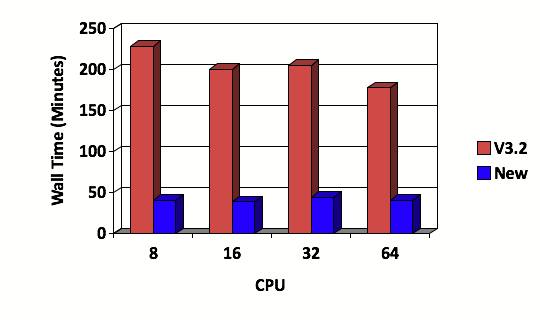
\includegraphics[scale=0.5]{big_case_performance}
\end{center}
}

%%%%%%%%%%%%%%%%%%%%%%%%%%%%%%%%%%%
\fst{}{
\begin{center}
~\\
~\\
~\\
~\\
~\\
{\huge{\color{red}Thank You}}\\
~\\
~\\
~\\
~\\
~\\
{\tiny{\color{blue}The NESL Mission is: \\
To advance understanding of weather, climate, atmospheric composition and processes;\\
To provide facility support to the wider community; and, \\
To apply the results to benefit society.\\}}
~\\
{\small{NCAR is sponsored by the National Science Foundation}}
\end{center}
}

\end{document}
